\documentclass{standalone}
\usepackage{tikz}
\usetikzlibrary{patterns, positioning}

\begin{document}
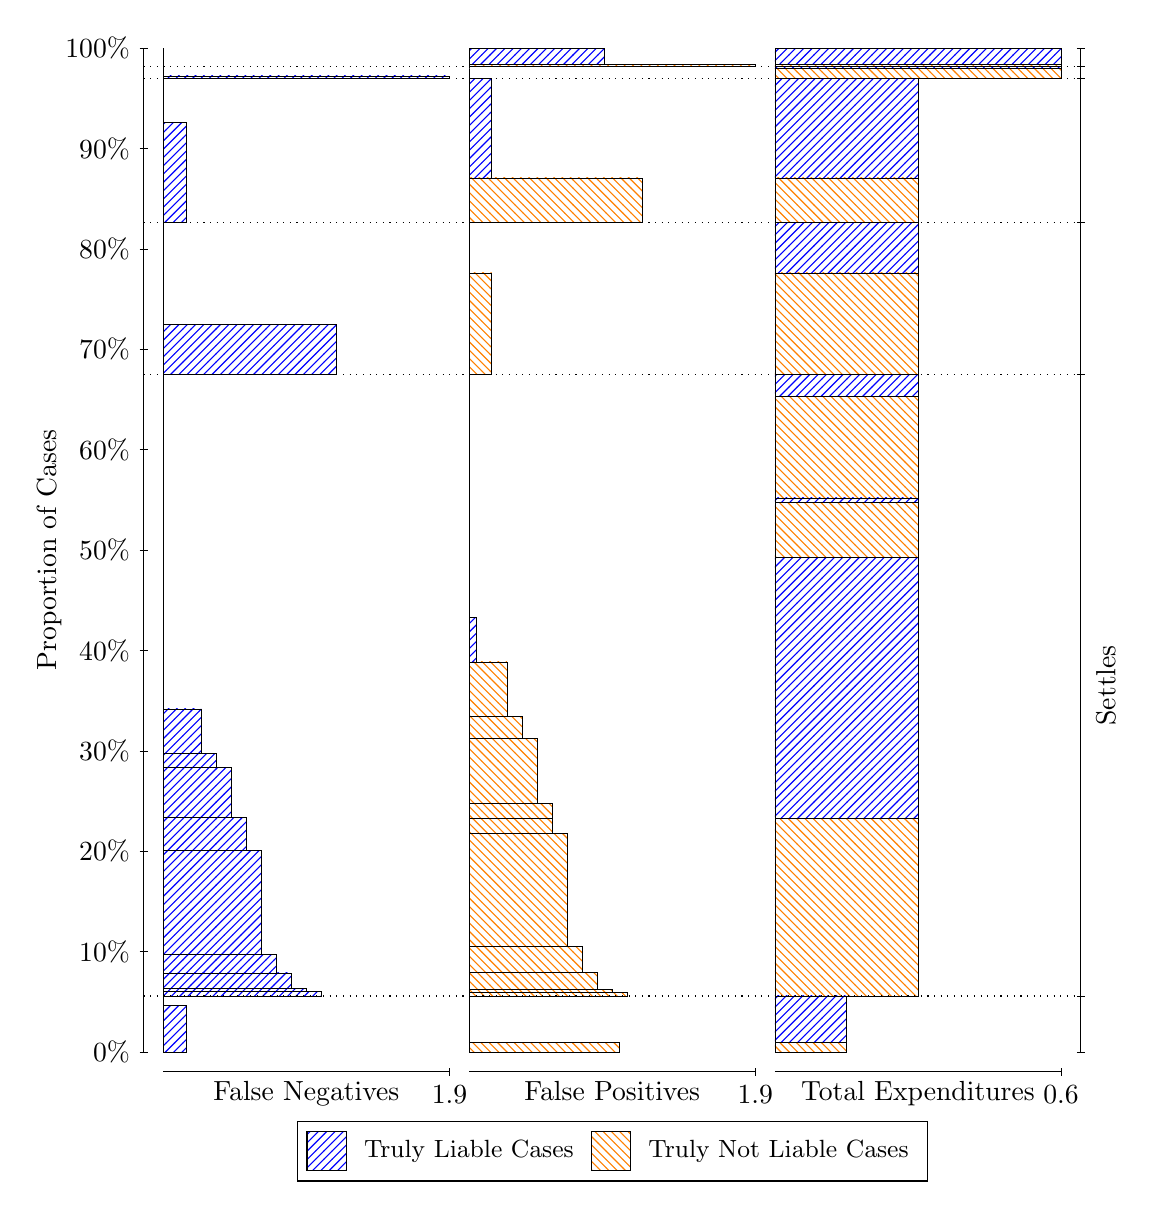
\begin{tikzpicture}
\draw[black, very thin] (1.5,1.75) -- (1.5,14.5);
\node[rotate=90, anchor=center] at (0.3, 8.125) {Proportion of Cases};
\draw[black, very thin] (1.45,1.75) -- (1.55,1.75);
\node[anchor=east] at (1.45, 1.75) {0\%};
\draw[black, very thin] (1.45,3.025) -- (1.55,3.025);
\node[anchor=east] at (1.45, 3.025) {10\%};
\draw[black, very thin] (1.45,4.3) -- (1.55,4.3);
\node[anchor=east] at (1.45, 4.3) {20\%};
\draw[black, very thin] (1.45,5.575) -- (1.55,5.575);
\node[anchor=east] at (1.45, 5.575) {30\%};
\draw[black, very thin] (1.45,6.85) -- (1.55,6.85);
\node[anchor=east] at (1.45, 6.85) {40\%};
\draw[black, very thin] (1.45,8.125) -- (1.55,8.125);
\node[anchor=east] at (1.45, 8.125) {50\%};
\draw[black, very thin] (1.45,9.4) -- (1.55,9.4);
\node[anchor=east] at (1.45, 9.4) {60\%};
\draw[black, very thin] (1.45,10.675) -- (1.55,10.675);
\node[anchor=east] at (1.45, 10.675) {70\%};
\draw[black, very thin] (1.45,11.95) -- (1.55,11.95);
\node[anchor=east] at (1.45, 11.95) {80\%};
\draw[black, very thin] (1.45,13.225) -- (1.55,13.225);
\node[anchor=east] at (1.45, 13.225) {90\%};
\draw[black, very thin] (1.45,14.5) -- (1.55,14.5);
\node[anchor=east] at (1.45, 14.5) {100\%};

\draw[black, very thin] (13.4,1.75) -- (13.4,14.5);
\draw[black, very thin] (13.35,1.75) -- (13.45,1.75);
\node[anchor=west] at (13.35, 1.75) {};
\draw[black, very thin] (13.35,2.4612) -- (13.45,2.4612);
\node[anchor=west] at (13.35, 2.4612) {};
\draw[black, very thin] (13.35,10.351) -- (13.45,10.351);
\node[anchor=west] at (13.35, 10.351) {};
\draw[black, very thin] (13.35,12.285) -- (13.45,12.285);
\node[anchor=west] at (13.35, 12.285) {};
\draw[black, very thin] (13.35,14.117) -- (13.45,14.117);
\node[anchor=west] at (13.35, 14.117) {};
\draw[black, very thin] (13.35,14.269) -- (13.45,14.269);
\node[anchor=west] at (13.35, 14.269) {};
\draw[black, very thin] (13.35,14.5) -- (13.45,14.5);
\node[anchor=west] at (13.35, 14.5) {};

\draw[black, very thin, pattern color=blue, pattern=north east lines] (1.75,1.75) rectangle (2.0368,2.3388);
\draw[black, very thin, pattern color=orange, pattern=north west lines] (1.75,2.3388) rectangle (1.75,2.4612);
\draw[black, very thin, pattern color=blue, pattern=north east lines] (1.75,2.4612) rectangle (3.7579,2.5192);
\draw[black, very thin, pattern color=blue, pattern=north east lines] (1.75,2.5192) rectangle (3.5667,2.5591);
\draw[black, very thin, pattern color=blue, pattern=north east lines] (1.75,2.5591) rectangle (3.3754,2.7537);
\draw[black, very thin, pattern color=blue, pattern=north east lines] (1.75,2.7537) rectangle (3.1842,2.9884);
\draw[black, very thin, pattern color=blue, pattern=north east lines] (1.75,2.9884) rectangle (2.993,4.3125);
\draw[black, very thin, pattern color=blue, pattern=north east lines] (1.75,4.3125) rectangle (2.8018,4.7285);
\draw[black, very thin, pattern color=blue, pattern=north east lines] (1.75,4.7285) rectangle (2.6105,5.3671);
\draw[black, very thin, pattern color=blue, pattern=north east lines] (1.75,5.3671) rectangle (2.4193,5.5434);
\draw[black, very thin, pattern color=blue, pattern=north east lines] (1.75,5.5434) rectangle (2.2281,6.1069);
\draw[black, very thin, pattern color=orange, pattern=north west lines] (1.75,6.1069) rectangle (1.75,10.351);
\draw[black, very thin, pattern color=blue, pattern=north east lines] (1.75,10.351) rectangle (3.9491,10.993);
\draw[black, very thin, pattern color=orange, pattern=north west lines] (1.75,10.993) rectangle (1.75,12.285);
\draw[black, very thin, pattern color=blue, pattern=north east lines] (1.75,12.285) rectangle (2.0368,13.553);
\draw[black, very thin, pattern color=orange, pattern=north west lines] (1.75,13.553) rectangle (1.75,14.117);
\draw[black, very thin, pattern color=blue, pattern=north east lines] (1.75,14.117) rectangle (5.3833,14.145);
\draw[black, very thin, pattern color=orange, pattern=north west lines] (1.75,14.145) rectangle (1.75,14.269);
\draw[black, very thin, pattern color=orange, pattern=north west lines] (1.75,14.269) rectangle (1.75,14.297);
\draw[black, very thin, pattern color=blue, pattern=north east lines] (1.75,14.297) rectangle (1.75,14.5);
\draw[black, very thin, pattern color=orange, pattern=north west lines] (5.6333,1.75) rectangle (7.5456,1.8724);
\draw[black, very thin, pattern color=blue, pattern=north east lines] (5.6333,1.8724) rectangle (5.6333,2.4612);
\draw[black, very thin, pattern color=orange, pattern=north west lines] (5.6333,2.4612) rectangle (7.6412,2.5089);
\draw[black, very thin, pattern color=orange, pattern=north west lines] (5.6333,2.5089) rectangle (7.45,2.5452);
\draw[black, very thin, pattern color=orange, pattern=north west lines] (5.6333,2.5452) rectangle (7.2588,2.7591);
\draw[black, very thin, pattern color=orange, pattern=north west lines] (5.6333,2.7591) rectangle (7.0675,3.0939);
\draw[black, very thin, pattern color=orange, pattern=north west lines] (5.6333,3.0939) rectangle (6.8763,4.5277);
\draw[black, very thin, pattern color=orange, pattern=north west lines] (5.6333,4.5277) rectangle (6.6851,4.7191);
\draw[black, very thin, pattern color=orange, pattern=north west lines] (5.6333,4.7191) rectangle (6.6851,4.9081);
\draw[black, very thin, pattern color=orange, pattern=north west lines] (5.6333,4.9081) rectangle (6.4939,5.7286);
\draw[black, very thin, pattern color=orange, pattern=north west lines] (5.6333,5.7286) rectangle (6.3026,6.0108);
\draw[black, very thin, pattern color=orange, pattern=north west lines] (5.6333,6.0108) rectangle (6.1114,6.705);
\draw[black, very thin, pattern color=blue, pattern=north east lines] (5.6333,6.705) rectangle (5.7289,7.2684);
\draw[black, very thin, pattern color=blue, pattern=north east lines] (5.6333,7.2684) rectangle (5.6333,10.351);
\draw[black, very thin, pattern color=orange, pattern=north west lines] (5.6333,10.351) rectangle (5.9202,11.643);
\draw[black, very thin, pattern color=blue, pattern=north east lines] (5.6333,11.643) rectangle (5.6333,12.285);
\draw[black, very thin, pattern color=orange, pattern=north west lines] (5.6333,12.285) rectangle (7.8325,12.85);
\draw[black, very thin, pattern color=blue, pattern=north east lines] (5.6333,12.85) rectangle (5.9202,14.117);
\draw[black, very thin, pattern color=orange, pattern=north west lines] (5.6333,14.117) rectangle (5.6333,14.241);
\draw[black, very thin, pattern color=blue, pattern=north east lines] (5.6333,14.241) rectangle (5.6333,14.269);
\draw[black, very thin, pattern color=orange, pattern=north west lines] (5.6333,14.269) rectangle (9.2667,14.297);
\draw[black, very thin, pattern color=blue, pattern=north east lines] (5.6333,14.297) rectangle (7.3544,14.5);
\draw[black, very thin, pattern color=orange, pattern=north west lines] (9.5167,1.75) rectangle (10.425,1.8724);
\draw[black, very thin, pattern color=blue, pattern=north east lines] (9.5167,1.8724) rectangle (10.425,2.4612);
\draw[black, very thin, pattern color=orange, pattern=north west lines] (9.5167,2.4612) rectangle (11.333,4.7191);
\draw[black, very thin, pattern color=blue, pattern=north east lines] (9.5167,4.7191) rectangle (11.333,8.0351);
\draw[black, very thin, pattern color=orange, pattern=north west lines] (9.5167,8.0351) rectangle (11.333,8.7293);
\draw[black, very thin, pattern color=blue, pattern=north east lines] (9.5167,8.7293) rectangle (11.333,8.7872);
\draw[black, very thin, pattern color=orange, pattern=north west lines] (9.5167,8.7872) rectangle (11.333,10.079);
\draw[black, very thin, pattern color=blue, pattern=north east lines] (9.5167,10.079) rectangle (11.333,10.351);
\draw[black, very thin, pattern color=orange, pattern=north west lines] (9.5167,10.351) rectangle (11.333,11.643);
\draw[black, very thin, pattern color=blue, pattern=north east lines] (9.5167,11.643) rectangle (11.333,12.285);
\draw[black, very thin, pattern color=orange, pattern=north west lines] (9.5167,12.285) rectangle (11.333,12.85);
\draw[black, very thin, pattern color=blue, pattern=north east lines] (9.5167,12.85) rectangle (11.333,14.117);
\draw[black, very thin, pattern color=orange, pattern=north west lines] (9.5167,14.117) rectangle (13.15,14.241);
\draw[black, very thin, pattern color=blue, pattern=north east lines] (9.5167,14.241) rectangle (13.15,14.269);
\draw[black, very thin, pattern color=orange, pattern=north west lines] (9.5167,14.269) rectangle (13.15,14.297);
\draw[black, very thin, pattern color=blue, pattern=north east lines] (9.5167,14.297) rectangle (13.15,14.5);
\draw[black, dotted] (1.5,2.4612) -- (13.4,2.4612);
\draw[black, dotted] (1.5,10.351) -- (13.4,10.351);
\draw[black, dotted] (1.5,12.285) -- (13.4,12.285);
\draw[black, dotted] (1.5,14.117) -- (13.4,14.117);
\draw[black, dotted] (1.5,14.269) -- (13.4,14.269);
\draw[black, very thin] (1.75,1.5) -- (5.3833,1.5);
\node[anchor=north] at (3.5667, 1.5) {False Negatives};
\draw[black, very thin] (5.3833,1.45) -- (5.3833,1.55);
\node[anchor=north] at (5.3833, 1.45) {1.9};

\draw[black, very thin] (5.6333,1.5) -- (9.2667,1.5);
\node[anchor=north] at (7.45, 1.5) {False Positives};
\draw[black, very thin] (9.2667,1.45) -- (9.2667,1.55);
\node[anchor=north] at (9.2667, 1.45) {1.9};

\draw[black, very thin] (9.5167,1.5) -- (13.15,1.5);
\node[anchor=north] at (11.333, 1.5) {Total Expenditures};
\draw[black, very thin] (13.15,1.45) -- (13.15,1.55);
\node[anchor=north] at (13.15, 1.45) {0.6};


\node[black, centered, rotate=90] at (13.72, 6.4059) {Settles};





\draw (7.449999999999999,1.5) node[draw=none] (baseCoordinate) {};
\begin{scope}[align=center]
        \matrix[scale=0.5, draw=black, below=0.5cm of baseCoordinate, nodes={draw}, column sep=0.1cm]{
            \node[rectangle, draw, minimum width=0.5cm, minimum height=0.5cm, pattern=north east lines, pattern color=blue] {}; &
            \node[draw=none, font=\small] (B) {Truly Liable Cases}; &
            \node[rectangle, draw, minimum width=0.5cm, minimum height=0.5cm, pattern=north west lines, pattern color=orange] {}; &
            \node[draw=none, font=\small] (B) {Truly Not Liable Cases}; \\
            };
\end{scope}

\end{tikzpicture}
\end{document}